%caseBldg

The first example is the Heating, Ventilation and Air Conditioning (HVAC) control of a 4-state model of a single zone in a building. Such a model is commonly used in literature for evaluation of predictive control algorithms \cite{Jain2016}. 
The control problem is similar to the example used in \cite{Raman14_MPCSTL}.
The control horizon is a 24 hour period.
The objective is to bring the zone temperature to a comfortable range, $[22,28]$ Celsius, when the zone is occupied during the hours 10-to-19. 
The specification is:
\begin{equation}
\label{eq:BldgSpec}
\formula = \always_{[10,19]}(\text{ZoneTemp} \in [22,28])
\end{equation}

\textit{Note:} For this particular specification, the maximum robustness is $3$, achievable by setting the room temperature at $25$C during the interval $[10,19]$.
Thus the problem can be solved by minimizing the cost $\sum_{10\leq k \leq 19}({x_4}_k-25)^2$ with linear constraints,
which is a problem-specific approach.
SOP, which is a general purpose technique, results in a robustness which is just $0.02\%$ smaller than the global optimum. 
Section~\ref{sec:ATCquad} shows a specification that cannot be trivially turned into a quadratic program.

\textbf{System dynamics.} The single-zone model, discretized at a sampling rate of 1 hour (which is common in building temperature control) is of the form:
\begin{equation}
\label{eq:bldg_dyn}
x_{k+1} = Ax_{k}+Bu_k+B_dd_k
\end{equation}
Here, $A$, $B$ and $B_d$ matrices are from the hamlab ISE model \cite{VanSchijndel2005}. $x \in \mathbb{R}^4$ is the state of the model, the $4^{th}$ element of which is the zone temperature, the others are auxiliary temperatures corresponding to other physical properties of the zone. 
The input to the system, $u \in \mathbb{R}^1$, is the heating/cooling energy. $b_d \in \mathbb{R}^3$ are disturbances (due to occupancy, outside temperature, solar radiation) assumed known a priori.
%perfect predictions of. Data for the disturbances is obtained for $1^{st}$ April 2000, which is our 24 hours of interest, from \cite{VanSchijndel2005}. 
The control problem we solve is of the form in \eqref{eq:general_ctrl}, with $\gamma$ and $\delta$ both set to zero (correspondingly, no cost for control in BluSTL), and $X=[0,50]^4$, $U=[-1000,2000]$.
%i.e. robustness (smooth, when applicable) is only in the objective, to be maximized. This allows for a fair comparison between the three methods. 
%With respect to the general control problem of \eqref{eq:general_ctrl}, the limits on the states are $X=[0,50]^4$ and on the inputs $U=[-1000,2000]$.

\begin{table}[tb]
\small
\begin{center}
\caption{{\small HVAC. Runtimes (mean and std deviation, in seconds) for Smooth Operator (SOP), BluSTL (BlS) and Simulated annealing (SA) over 100 runs with random initial states. BluSTL (R) could not find satisfying trajectories.}}
\vspace{-5pt}
\label{tbl:time_performance_bldg}
\begin{tabular} {|c|c|c|c|}
	\hline
	BlS (B) & SOP (B) & SOP (R) & SA (R) \\ \hline
	 $0.041 \pm 0.002$ &  $\mathbf{0.014 \pm 0.002}$  &  $2.532 \pm 0.26$ & $8.56 \pm 0.31$ \\ \hline 
\end{tabular}	
\end{center}
\vspace{-10pt}
\end{table}



\textbf{Results.} For comparison across all methods, we run 100 instances of the problem, starting from random initial states $x_0 \in [20,21]^4$. SA, R-SQP and SOP are initialized with the same initial input sequences $\mathbf{u}$. 
The final trajectories after optimization are shown in Fig.\ref{fig:ZoneTemp}, for $x_0 = [21,21,21,21]'$. To reduce clutter, trajectories from SA and R-SQP in mode (B) are not shown.

\begin{figure}[t]
\centering
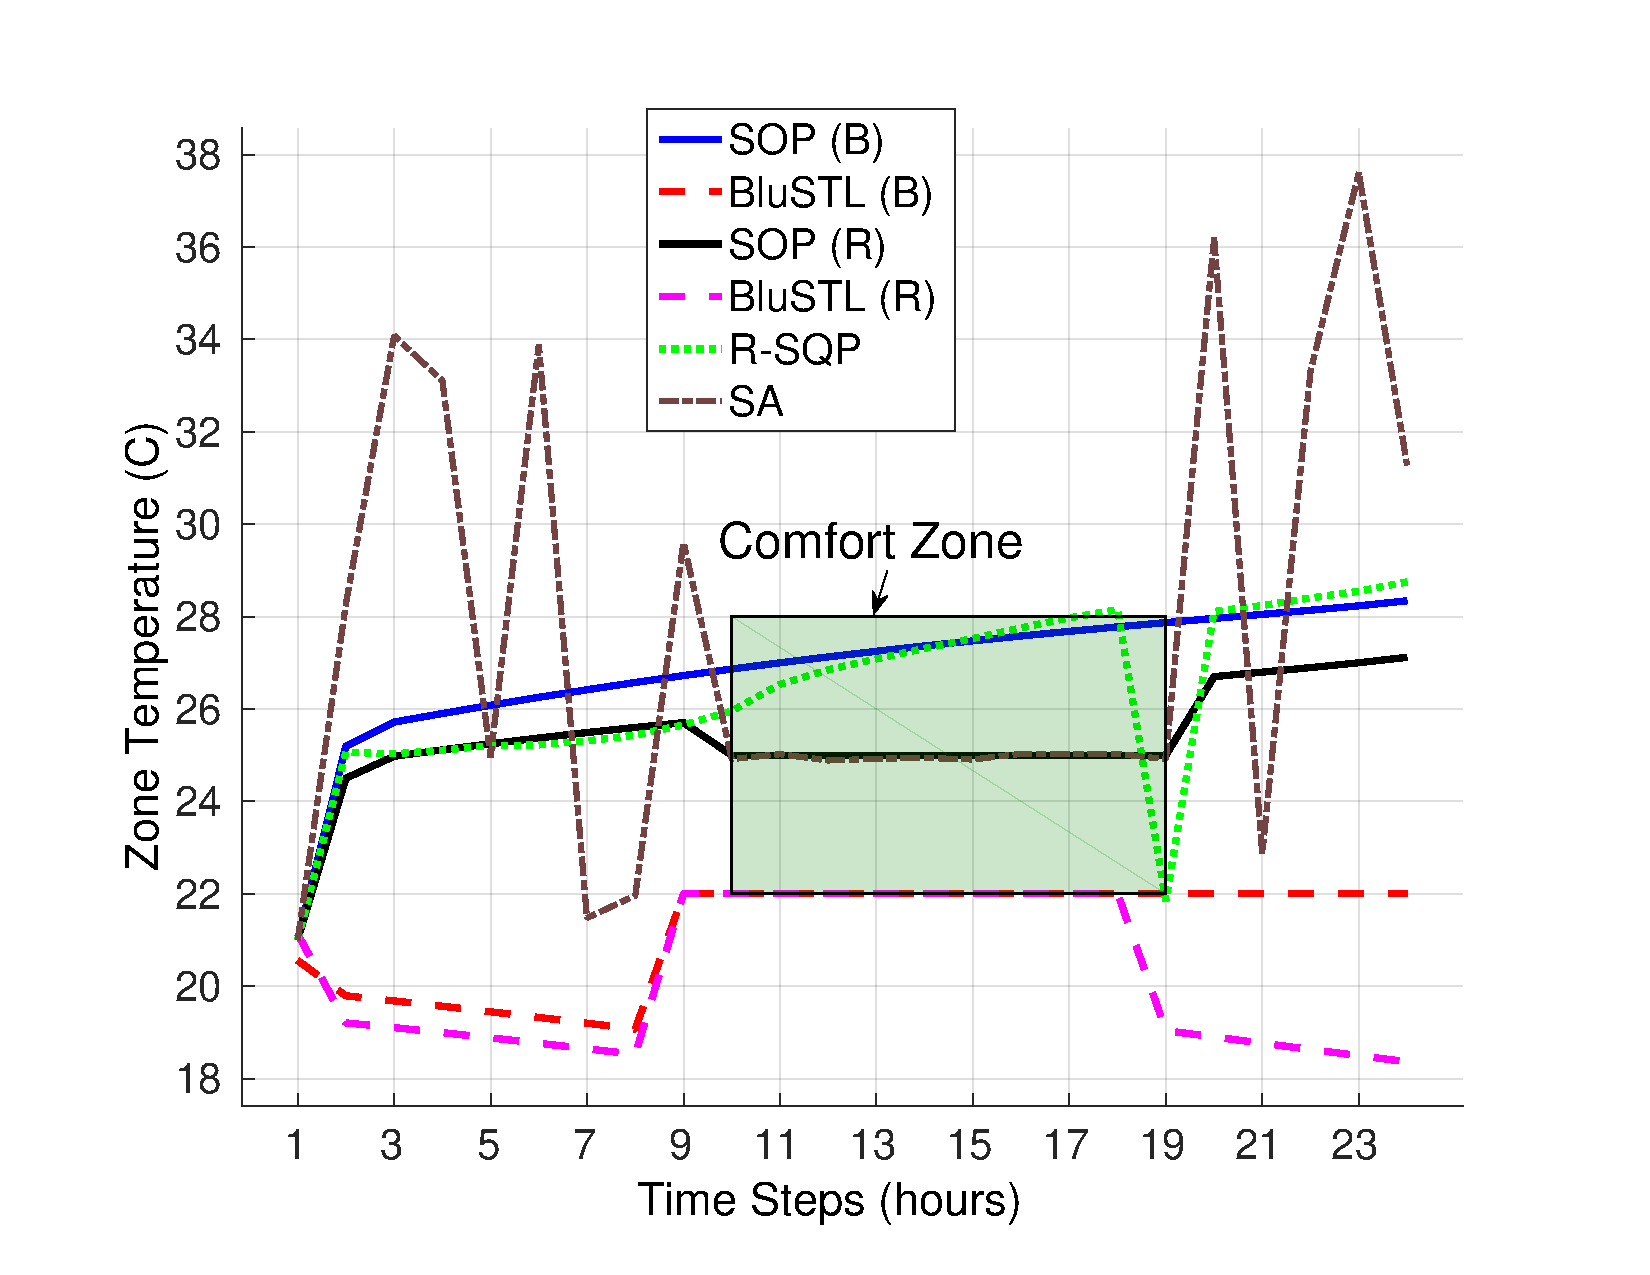
\includegraphics[width=0.49\textwidth]{figures/ZoneTempFinal}
\vspace{-20pt}
\caption{\small{Zone temperatures. The green rectangle shows the comfortable temperature limit of 22-28 C, applicable during time steps 10-19 (when the building is occupied). Color in online version.}}
\label{fig:ZoneTemp}
\vspace{-10pt}
\end{figure}


\textbf{Analysis.} 
In Boolean mode, SOP, BluSTL, and SA all find satisfying trajectories across all 100 instances, while R-SQP does not find one for any run and always exits at a local minimum. 
Execution times for SOP and BluSTL are shown in Table \ref{tbl:time_performance_bldg}, while the runtimes for SA (B) are $3.7 \pm 2.3s$.
 R-SQP has run-times in the order of minutes. 
 %This is because of Matlab's failed attempts at approximating a gradient that does not exist. %say whaaaa???
 
In Robust mode, SOP and SA both result in trajectories that satisfy $\formula$, with an average robustness of $2.99$ and $2.88$ respectively. On the other hand, R-SQP often returns violating trajectories (average $\rob_{\formula} = -0.1492$). 
Somewhat surprisingly, BluSTL does not manage to find a satisfying trajectory (average $\rho=-2.71$) for any of the 100 runs. 
One particular instance is shown in Fig. \ref{fig:ZoneTemp}. 
%This could be because the MILP encoding of robustness for this example results in the solver finding local minima which have negative robustness. 
As shown in Table \ref{tbl:time_performance_bldg}, SOP takes $2.5s$ on average.
SA(R) takes $8.56 \pm 0.31s$ on average. 
R-SQP again takes minutes on average to return non-satisfying trajectories across all 100 runs. 
%This is possibly due to the lack of existence of a gradient along certain directions, as seen in example \ref{ex:cluster nondiff}.

%\ypcomment{Move to after spec.}

%, while SA gets to a value $3.8\%$ less than the global optima. 
%We use this example to illustrate the applicability of our method, as well as its performance, while adding a word of caution against the use of gradient descent for maximizing the true robustness.
%, even while the gradient of robustness exists \textit{almost everywhere}. 
%In the following example, we take a specification which cannot be trivially turned into a quadratic-program. %without adding tighter constraints than the specification asks for (or binary variables).

\subsubsection{Shrinking horizon implementation} 
\label{sec:online}
%\textbf{Online implementation.} 
SOP can also be applied online in a shrinking horizon fashion similar to \cite{Raman14_MPCSTL}. 
The control horizon in Eq. \eqref{eq:general_ctrl} equals the formula horizon $N$. %, and evaluating $\srob$ requires a trajectory of length at most $N$. 
For each time step $k=0,\dotsc,N$, problem~\eqref{eq:general_ctrl} is solved while constraining the previously applied inputs and states (for times steps $<k$) to their actual values. 
In this scheme, the length of the optimization remains $N$, but the number of free variables keeps on shrinking as $k$ increases. 
For initializing SOP at each time step, the sequence of inputs computed at time $k-1$ is used as a feasible solution for the optimization at time $k$. 
We implemented this scheme for the HVAC control problem with additional unknown disturbances in $d_k$ term of Eq.~\eqref{eq:bldg_dyn}.
%begin{equation}
%\label{eq:bldg_dyn_noisy}
%$x_{k+1} = Ax_{k}+Bu_k+B_dd_k+B_dw_k$$
%\end{equation}
The disturbances are in the form random variable centred around the known $d_k$ with a width of $10\%$ of element wise magnitude of $d_k$. This can be thought of as prediction errors in the disturbances like solar radiation and outside temperature. Over 100 runs with random initial states as before, the online application of SOP (in \textit{robust} mode) resulted in an average robustness value of $2.91$. In terms of execution time, the first iteration takes times of the order of those in table \ref{tbl:time_performance_bldg}, and subsequent iterations take a fraction of that time (average for one instance $0.0151s$). This is because we re-use the input sequence at time $k-1$ as an initial guess for the solver at time $k$. Since at the initial time step we have achieved near global robustness maxima, the subsequent SQP optimizations terminate much faster while the formulation takes into account change in the state due to disturbance values by making small changes to the input sequence being computed at time $k>0$. The high value of average robustness and the small execution time per iteration show the applicability of SOP as an online closed loop control method. 
